% -----------------
% abnTeX2: Modelo de Trabalho Academico (tese de doutorado, dissertacao de
% mestrado e trabalhos monograficos em geral) em conformidade com 
% ABNT NBR 14724:2011: Informacao e documentacao - Trabalhos academicos -
% Apresentacao
% -----------------

\documentclass[
	% -- opções da classe memoir --
	12pt,                     % tamanho da fonte
	openright,                % capítulos começam em pág ímpar (insere página vazia caso preciso)
	oneside,                  % twoside para impressão em verso e anverso. Oposto a oneside
	a4paper,                  % tamanho do papel. 
  % -- opções da classe abntex2 --
	% chapter=TITLE,          % títulos de capítulos convertidos em letras maiúsculas
	% section=TITLE,          % títulos de seções convertidos em letras maiúsculas
	% subsection=TITLE,       % títulos de subseções convertidos em letras maiúsculas
	% subsubsection=TITLE,    % títulos de subsubseções convertidos em letras maiúsculas
  % -- opções do pacote babel --
	english,                  % idioma adicional para hifenização
	% french,                 % idioma adicional para hifenização
	% spanish,                % idioma adicional para hifenização
	brazil                    % o último idioma é o principal do documento
]{abntex2}

% --- 
% Pacotes básicos 
\usepackage{lmodern}          % Usa a fonte Latin Modern		>
\usepackage[T1]{fontenc}      % Selecao de codigos de fonte.
\usepackage[utf8]{inputenc}   % Codificacao do documento (conversão automática dos acentos)
\usepackage{lastpage}         % Usado pela Ficha catalográfica
\usepackage{indentfirst}      % Indenta o primeiro parágrafo de cada seção.
\usepackage{color}            % Controle das cores
\usepackage{graphicx}         % Inclusão de gráficos
\usepackage{microtype}        % para melhorias de justificação
\usepackage[dvipsnames]{xcolor}
\usepackage[portuges]{datetime2}
% \DTMlangsetup[portuges]{showdayofmonth=false}
		
% ---
% Pacotes adicionais, usados apenas no âmbito do Modelo Canônico do abnteX2
\usepackage{lipsum}                           % para geração de dummy text

% ---
% Pacotes de citações
\usepackage[brazilian,hyperpageref]{backref}  % Paginas com as citações na bibl
\usepackage[alf]{abntex2cite}                 % Citações padrão ABNT

% --- 
% CONFIGURAÇÕES DE PACOTES

% Configurações do pacote backref
% Usado sem a opção hyperpageref de backref
\renewcommand{\backrefpagesname}{Citado na(s) página(s):~}

% Texto padrão antes do número das páginas
\renewcommand{\backref}{}

% Define os textos da citação
\renewcommand*{\backrefalt}[4]{
	\ifcase #1
		Nenhuma citação no texto.
	\or
		Citado na página #2.
	\else
		Citado #1 vezes nas páginas #2.
	\fi}

% Novos comandso
\newcommand{\cp}[1]{{\color{orange} [@CopyAndPaste] #1}}
	
% ---
% Informações de dados para CAPA e FOLHA DE ROSTO

\titulo{Sistema de Monitoramento de Qualidade de Vacinas}
\autor{Henrique Martins Miranda}
\local{Campina Grande}
\data{\the\year{}}
\orientador{Ruan Delgado Gomes}
\newcommand{\instituto}{
  Instituto Federal de Educação, Ciência e Tecnologia\\
  da Paraíba - Campus Campina Grande\\
  Curso Superior de Tecnologia em Telemática
}
\tipotrabalho{Trabalho de conclusão de curso}
% O preambulo deve conter o tipo do trabalho, o objetivo, 
% o nome da instituição e a área de concentração 
\preambulo{Trabalho de conclusão de curso, Instituto Federal de Educação, 
Ciência e Tecnologia da Paraíba - Campus Campina Grande, 
curso superior de Tecnologia em Telemática}

\renewcommand{\imprimircapa}{
  \begin{capa}
    \center
    
    \begin{figure}
      \begin{center}
        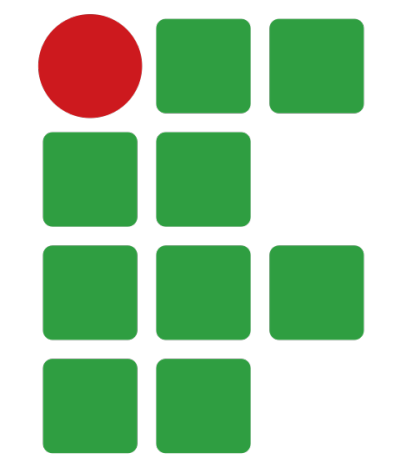
\includegraphics[width=1.8cm]{./assets/logo-ifpb.png}
      \end{center}
    \end{figure}
    
    \ABNTEXchapterfont \large \MakeUppercase{\instituto}
    
    \vspace*{2.5cm}
    
    \ABNTEXchapterfont \large \MakeUppercase{\imprimirautor}
    
    \vfill
    \begin{center}
      \ABNTEXchapterfont \bfseries \large \MakeUppercase{\imprimirtitulo}
    \end{center}
    \vfill
    % \vspace*{6.25cm}

    \large \imprimirlocal
    \par
    \large \imprimirdata
    \vspace*{1cm}
  \end{capa}
}

	
% ---
% Configurações de aparência do PDF final

\definecolor{blue}{RGB}{41,5,195}  % alterando o aspecto da cor azul

% informações do PDF
\makeatletter
\hypersetup{
  % pagebackref=true,
  pdftitle={\@title}, 
  pdfauthor={\@author},
  pdfsubject={\imprimirpreambulo},
  pdfcreator={LaTeX with abnTeX2},
  pdfkeywords={abnt}{latex}{abntex}{abntex2}{trabalho acadêmico}, 
  colorlinks=true,          % false: boxed links; true: colored links
  linkcolor=blue,           % color of internal links
  citecolor=blue,           % color of links to bibliography
  filecolor=magenta,        % color of file links
  urlcolor=blue,
  bookmarksdepth=4
}
\makeatother

% --- 
% Espaçamentos entre linhas e parágrafos 

\setlength{\parindent}{1.3cm} % O tamanho do parágrafo

% Controle do espaçamento entre um parágrafo e outro:
\setlength{\parskip}{0.2cm} % Tente também \onelineskip

\makeindex  % Compila o indice

% ---
% Início do documento
\begin{document}
\frenchspacing  % Retira espaço extra obsoleto entre as frases.

% ---
% ELEMENTOS PRÉ-TEXTUAIS
% ---
\pretextual
\imprimircapa
\imprimirfolhaderosto*

% Isto é um exemplo de Ficha Catalográfica, ou ``Dados internacionais de
% catalogação-na-publicação''. Você pode utilizar este modelo como referência. 
% Porém, provavelmente a biblioteca da sua universidade lhe fornecerá um PDF
% com a ficha catalográfica definitiva após a defesa do trabalho. Quando estiver
% com o documento, salve-o como PDF no diretório do seu projeto e substitua todo
% o conteúdo de implementação deste arquivo pelo comando abaixo:
%
% \begin{fichacatalografica}
%     \includepdf{fig_ficha_catalografica.pdf}
% \end{fichacatalografica}

\begin{fichacatalografica}
  \vspace*{\fill}                 % Posição vertical
  \hrule                          % Linha horizontal
  \begin{center}                  % Minipage Centralizado
    \begin{minipage}[c]{12.5cm}   % Largura

      \imprimirautor

      \hspace{0.5cm} \imprimirtitulo  / \imprimirautor. --
      \imprimirlocal, \imprimirdata-

      \hspace{0.5cm} \pageref{LastPage} p. : il. (algumas color.) ; 30 cm.\\

      \hspace{0.5cm} \imprimirorientadorRotulo~\imprimirorientador\\

      \hspace{0.5cm}
      \parbox[t]{\textwidth}{\imprimirtipotrabalho~--~\imprimirinstituicao,
        \imprimirdata.}\\

      \hspace{0.5cm}
      1. Palavra-chave1.
      2. Palavra-chave2.
      I. Orientador.
      II. Universidade xxx.
      III. Faculdade de xxx.
      IV. Título\\

      \hspace{8.75cm} CDU 02:141:005.7\\

    \end{minipage}
  \end{center}
  \hrule
\end{fichacatalografica}
       % Ficha bibliografica
% \begin{errata}
  Elemento opcional da \citeonline[4.2.1.2]{NBR14724:2011}. Exemplo:

  \vspace{\onelineskip}

  FERRIGNO, C. R. A. \textbf{Tratamento de neoplasias ósseas apendiculares com
  reimplantação de enxerto ósseo autólogo autoclavado associado ao plasma
  rico em plaquetas}: estudo crítico na cirurgia de preservação de membro em
  cães. 2011. 128 f. Tese (Livre-Docência) - Faculdade de Medicina Veterinária e
  Zootecnia, Universidade de São Paulo, São Paulo, 2011.

  \begin{table}[htb]
    \center
    \footnotesize
    \begin{tabular}{|p{1.4cm}|p{1cm}|p{3cm}|p{3cm}|}
      \hline
      \textbf{Folha} & \textbf{Linha} & \textbf{Onde se lê} & \textbf{Leia-se} \\
      \hline
      1              & 10             & auto-conclavo       & autoconclavo     \\
      \hline
    \end{tabular}
  \end{table}

\end{errata}
        % Errata
% Isto é um exemplo de Folha de aprovação, elemento obrigatório da NBR
% 14724/2011 (seção 4.2.1.3). Você pode utilizar este modelo até a aprovação
% do trabalho. Após isso, substitua todo o conteúdo deste arquivo por uma
% imagem da página assinada pela banca com o comando abaixo:
%
% \includepdf{folhadeaprovacao_final.pdf}
%

\begin{folhadeaprovacao}
  \begin{center}
    {\ABNTEXchapterfont\large\imprimirautor}

    \vspace*{\fill}\vspace*{\fill}
    \begin{center}
      \ABNTEXchapterfont \bfseries \Large \imprimirtitulo
    \end{center}
    \vspace*{\fill}

    \hspace{.45\textwidth}
    \begin{minipage}{.5\textwidth}
      \imprimirpreambulo
    \end{minipage}
    \vspace*{\fill}
    
    % Trabalho aprovado. \imprimirlocal, \today:
  \end{center}

  \assinatura{\textbf{\imprimirorientador} \\ Orientador}
  \assinatura{\textbf{Professor} \\ Membro da Banca}
  \assinatura{\textbf{Professor} \\ Membro da Banca}

  \begin{center}
    \vspace*{0.5cm}
    {\large\imprimirlocal}
    \par
    {\large\imprimirdata}
    \vspace*{1cm}
  \end{center}

\end{folhadeaprovacao}
      % Folha de aprovação
% \begin{dedicatoria}
  \vspace*{\fill}
  \centering
  \noindent
  \textit{Este trabalho é dedicado às crianças adultas que,\\
    quando pequenas, sonharam em se tornar cientistas.} \vspace*{\fill}
\end{dedicatoria}
    % Dedicatória
\begin{agradecimentos}
  
\end{agradecimentos}
        % Agradecimentos
% \begin{epigrafe}
  \vspace*{\fill}
  \begin{flushright}
    \textit{}
  \end{flushright}
\end{epigrafe}
      % Epígrafe
% resumo em português
\setlength{\absparsep}{18pt} % ajusta o espaçamento dos parágrafos do resumo
\begin{resumo}
  \cp{
    O armazenamento é um dos componentes mais importantes da cadeia de 
    distribuição de vacinas, principalmente pela sensibilidade delas a variações 
    de temperatura, que podem ocasionar diminuição da sua eficácia. Considerando 
    isso, existe uma necessidade de manter constante monitoramento dessa variável, 
    afim de garantir que o produto final venha a manter suas característica 
    originais e a eficiência esperada. Esse trabalho apresenta uma solução baseada em Internet das Coisas, usando comunicação sem fio de baixa potência, para monitorar a qualidade de vacinas, por meio das medidas de temperatura e umidade nos locais de armazenamento. Os dados coletados são organizados em um banco de dados, podendo ser acessados por sistemas decisórios afim de avaliar a qualidade da vacina antes de sua aplicação, evitando problemas em decorrência de problemas de armazenamento.
  }

  \textbf{Palavras-chaves}: Monitoramento. Vacinas. IoT. LoRa.
\end{resumo}

% resumo em inglês
\begin{resumo}[Abstract]
  \begin{otherlanguage*}{english}
    This is the english abstract.

    \vspace{\onelineskip}

    \noindent
    \textbf{Key-words}: Monitoring. vacaciones. IoT. LoRa.
  \end{otherlanguage*}
\end{resumo}
     % Resumos
% ---
% Lista de ilustrações
\pdfbookmark[0]{\listfigurename}{lof}
\listoffigures*
\cleardoublepage

% ---
% Lista de tabelas
\pdfbookmark[0]{\listtablename}{lot}
\listoftables*
\cleardoublepage

% ---
% Lista de abreviaturas e siglas
\begin{siglas}
  \item[ABNT] Associação Brasileira de Normas Técnicas
  \item[abnTeX] ABsurdas Normas para TeX
\end{siglas}

% ---
% Lista de símbolos
\begin{simbolos}
  \item[$ \Gamma $] Letra grega Gama
  \item[$ \Lambda $] Lambda
  \item[$ \zeta $] Letra grega minúscula zeta
  \item[$ \in $] Pertence
\end{simbolos}
         % Listas

% ---
% Sumario
\pdfbookmark[0]{\contentsname}{toc}
\tableofcontents*
\cleardoublepage

% ---
% ELEMENTOS TEXTUAIS
% ---
\textual

% ---
% Introdução (exemplo de capítulo sem numeração, mas presente no Sumário)
\chapter[Introdução]{Introdução}
\label{cap:intro}
% ---

A saúde é um fator de suma importância para todos os seres vivos, ele é um problema científico, tecnológico, político, prático e filosófico que refere-se a um estado completo de bem estar físico, emocional, social, intelectual e espiritual \cite{almeida2011saude}. 

Segundo o artigo 196 \cite{de2013direito} da Constituição Federal Brasileira a saúde é um direito de todos e dever do Estado garantir medidas políticas sociais e econômicas que visam à diminuição do risco de doenças e de outros agravamentos e ao acesso universal e imparcial às ações e serviços para a sua promoção, proteção e recuperação.

Para garantirmos nossa saúde, precisamos cuidar do nosso corpo e mente, para isto, uma ferramenta que podemos contar são os imunobiológicos, como as vacinas e os soros, diferente de remédios que ajudam no tratamento de pessoas doentes, as imunobiológicos são uma preparação biológica que fornece imunidade total ou parcial de uma determinada doença autoimune para um indivíduo saudável. As vacinas e os soros se diferem pela sua forma de imunização, as vacinas fornece uma imunização ativa, estimulando o nosso organismo na produção de anticorpos, os soros fornecem uma imunização passiva, provendo os anticorpos para o nosso organismo que foram produzidos  em outros organismo \cite{soma2018tratamento}.

Contudo, os imunobiológicos requerem um cuidado elevado para manter a qualidade e sua eficiência, um dos fatores é que são produtos termolábeis, ou seja, se deterioram após determinado tempo expostos a variações de temperaturas e umidade, portanto, é imprescindível assegurar que seu ambiente de armazenagem mantenha uma temperatura e umidade consante \cite{ministerio2001manual} para garantir uma longevidade maior para o produto. Para este propósito, existem as redes de frio, um processo desenvolvido pelo Programa Nacional de Imunizações, PNI, de conversação, armazenamento e transporte dos medicamentos, objetivando as condições adequadas dos mesmos, mantendo suas características iniciais \cite{ministerio2001manual}.

No ano de 2014, foi relatado em um estudo \cite{oliveira2014avaliaccao} que a qualidade de conservação das vacinas não eram adequadas em boa parte dos municípios da macroregião Oeste de Minas Gerais, alguns dos motivos citados foram a má gestão dos refrigeradores, falhas no minitoramento da temperatura e insuficiência de recusos humanos.



\begin{itemize}
  \item \todo{Falar sobre dificuldade no controle de qualidade}
  \item \todo{Falar da IoT}
  \item \todo{Falar da solução proposta}
\end{itemize}

\section{O Programa Nacional de Imunizações}
\label{intro:justificativa}

Com o sucesso da Campanha de Erradicação da Varíola, CEV, iniciada em 1965, tendo seu fim em 1973 \cite{muniz2011memorias}, amplificou dentro do Ministério da Saúde maiores investimento no controle de doenças autoimune, dando um impulso na criação do PNI \cite{temporao2003programa}. O PNI foi fundado com objetivo de controlar e erradicar as doenças imunopreveníveis, através de ações metalizadas de vacinação da população. Em 1980 foi realizada a primeira campanha de vacinação da poliomielite e desde então foram realizadas diversas campanhas, tais como a da rubéola, sarampo, tuberculose febre amarela entre outras \cite{temporao2003programa,ministerio2001manual}.

De acordo com a Lei n.º 6.259 de 30 de outubro de 1975, regularizada pelo Decreto nº 78.231 em 1976, certificar o PNI, sobre a responsabilidade do Ministerio da Sáude e define as seguintes competências \cite{ministerio2001manual}:
  \begin{itemize}
    \item implantar e implementar as ações do Programa, relacionadas com as vacinações de caráter obrigatório;
    \item  estabelecer critérios e prestar apoio técnico e financeiro à elaboração, implantação e implementação dos programas de vacinação a cargo das secretarias de saúde das unidades federadas;
    \item estabelecer normas básicas para a execução das vacinações;
    \item supervisionar, controlar e avaliar a execução das vacinações no território nacional, principalmente o desempenho dos órgãos das Secretarias de Saúde, encarregados dos programas de vacinação.
  \end{itemize}
% ---
\section{Justificativa e Relevância do Trabalho}
\label{intro:justificativa}



\begin{itemize}
  \item \todo{Falar das perdas e prejuizos}
  \item \todo{Falar dos beneficios ao usar um aplicão desse porte}
\end{itemize}

% ---
\section{Objetivos}
\label{intro:objetivos}

\subsection{Objetivo Geral}
\label{intro:objetivos:geral}
Construir uma arquitetura baseada em conceitos de IoT visando o monitoramento de temperatura e umidade de imunobiológicos para auxiliar funcionários da saúde, garantindo melhores condições para a vacinação da população frente a incidência de doenças.

\subsection{Objetivos Específicos}
\label{intro:objetivos:especificos}
\begin{itemize}
  \item Construir um protótipo inicial para coleta da temperatura e umidade nos ambientes de armazenagens dos imunobiológicos.
  \item Implementar um servidor para a armazenagem dos dados coletados e posteriormente fornecer históricos das temperaturas e umidade ao aplicativo móvel.
  \item Desenvolver um aplicativo móvel para fornecer uma interface amigável para os usuários auxiliando no controle de qualidade dos produtos.
  \item Realizar testes e análises dos dados de transmissões a fim de garantir a confiabilidade das temperaturas e umidade coletadas.
\end{itemize}

% ---
\section{Metodologia}
\label{intro:metodologia}
No intuito de alcançar os objetivos pretendidos, a metodologia utilizada neste trabalho
foi composta pelas seguintes etapas:

\begin{itemize}
  \item \todo{Adicionar os pontos}.
\end{itemize}

% ---
\section{Organização do Documento}
\label{intro:organizacao}
\hm{A ser feito quando o documento tiver pronto}

% ---
% PARTE
\part{Preparação da pesquisa}

% ---
% Capitulo com exemplos de comandos inseridos de arquivo externo 
\include{abntex2-modelo-include-comandos}

% ---
% PARTE
% ---
\part{Referenciais teóricos}

% ---
% Capitulo de revisão de literatura
\chapter{Lorem ipsum dolor sit amet}

% ---
\section{Aliquam vestibulum fringilla lorem}

\lipsum[1]

\lipsum[2-3]

% ---
% PARTE
\part{Resultados}

% ---
% primeiro capitulo de Resultados
\chapter{Lectus lobortis condimentum}

% ---
\section{Vestibulum ante ipsum primis in faucibus orci luctus et ultrices
  posuere cubilia Curae}

\lipsum[21-22]

% ---
% segundo capitulo de Resultados
\chapter{Nam sed tellus sit amet lectus urna ullamcorper tristique interdum
  elementum}

% ---
\section{Pellentesque sit amet pede ac sem eleifend consectetuer}

\lipsum[24]
 % Capítulos

% ---
% Finaliza a parte no bookmark do PDF
% para que se inicie o bookmark na raiz
% e adiciona espaço de parte no Sumário
% ---

%\phantompart

% Conclusão (outro exemplo de capítulo sem numeração e presente no sumário)
\chapter{Considerações Finais}
\label{cap:conlusao}


\section{Sugestões para Trabalhos Futuros}
\label{sec:futuros}

% ---
% ELEMENTOS PÓS-TEXTUAIS
% ---
\postextual

\bibliography{abntex2-modelo-references}        % Referências bibliográficas

% ---
% Glossário
% Consulte o manual da classe abntex2 para orientações sobre o glossário.
% \glossary

\begin{apendicesenv}
  \partapendices  % Imprime uma página indicando o início dos apêndices

  % ---
  \chapter{Um Apêndice}
  \label{ape:apendiceI}
  Para criar um novo apêndice utilize o comando chapter, lembre de utilizar label para referenciar.

\end{apendicesenv}
   % Apêndices
\begin{anexosenv}
  \partanexos % Imprime uma página indicando o início dos anexos

  % ---
  \chapter{Morbi ultrices rutrum lorem.}

  \lipsum[30]

\end{anexosenv}
      % Anexos

%---
% INDICE REMISSIVO
% \phantompart
\printindex

\end{document}
